
\section{Code implementation control}

We implemented the code in 3D ground motion simulation code called Hercules. In order to make sure that the code works as expected we developed a 1D finite element site response analysis code and verify it with DEEPSOIL. Later on, we ran a problem in 1D and a simplified 3D version. In simplified 3D version every factors remain 3D unless we give the force at the bottom of the domain in 1 direction which makes it similar to 1D.  We compare the equivalent linear code implementation in both 1D and 3D in 3 different domain. 

 
\begin{itemize}
  \item Homogenous
  \item Layered - 2 Layeres
  \item Layered - 3 Layeres
\end{itemize}

The results shows the code accurately extract the strain and update the materials for different iteration. Fig.~\ref{fig:comparison_1D_3D_3models} shows these 3 domains. 

 \begin{figure}[H]
    \centering
    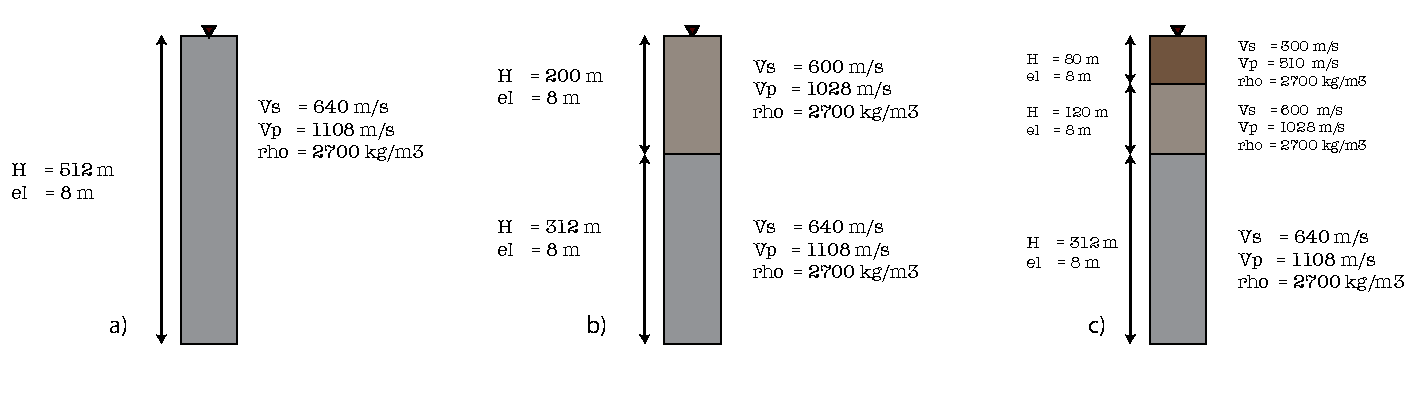
\includegraphics[width=\textwidth]{figures/pdf/comparison_1D_3D_3models.pdf}
    \caption{Study domain for comparison of 3D and 1D equivalent linear method for idealized 3D domain.}
    \label{fig:comparison_1D_3D_3models}
\end{figure}

The results for these domains for 3 iteration are shown in Fig.~\ref{fig:comparison_1D_3D_3models_results}

 \begin{figure}[H]
    \centering
    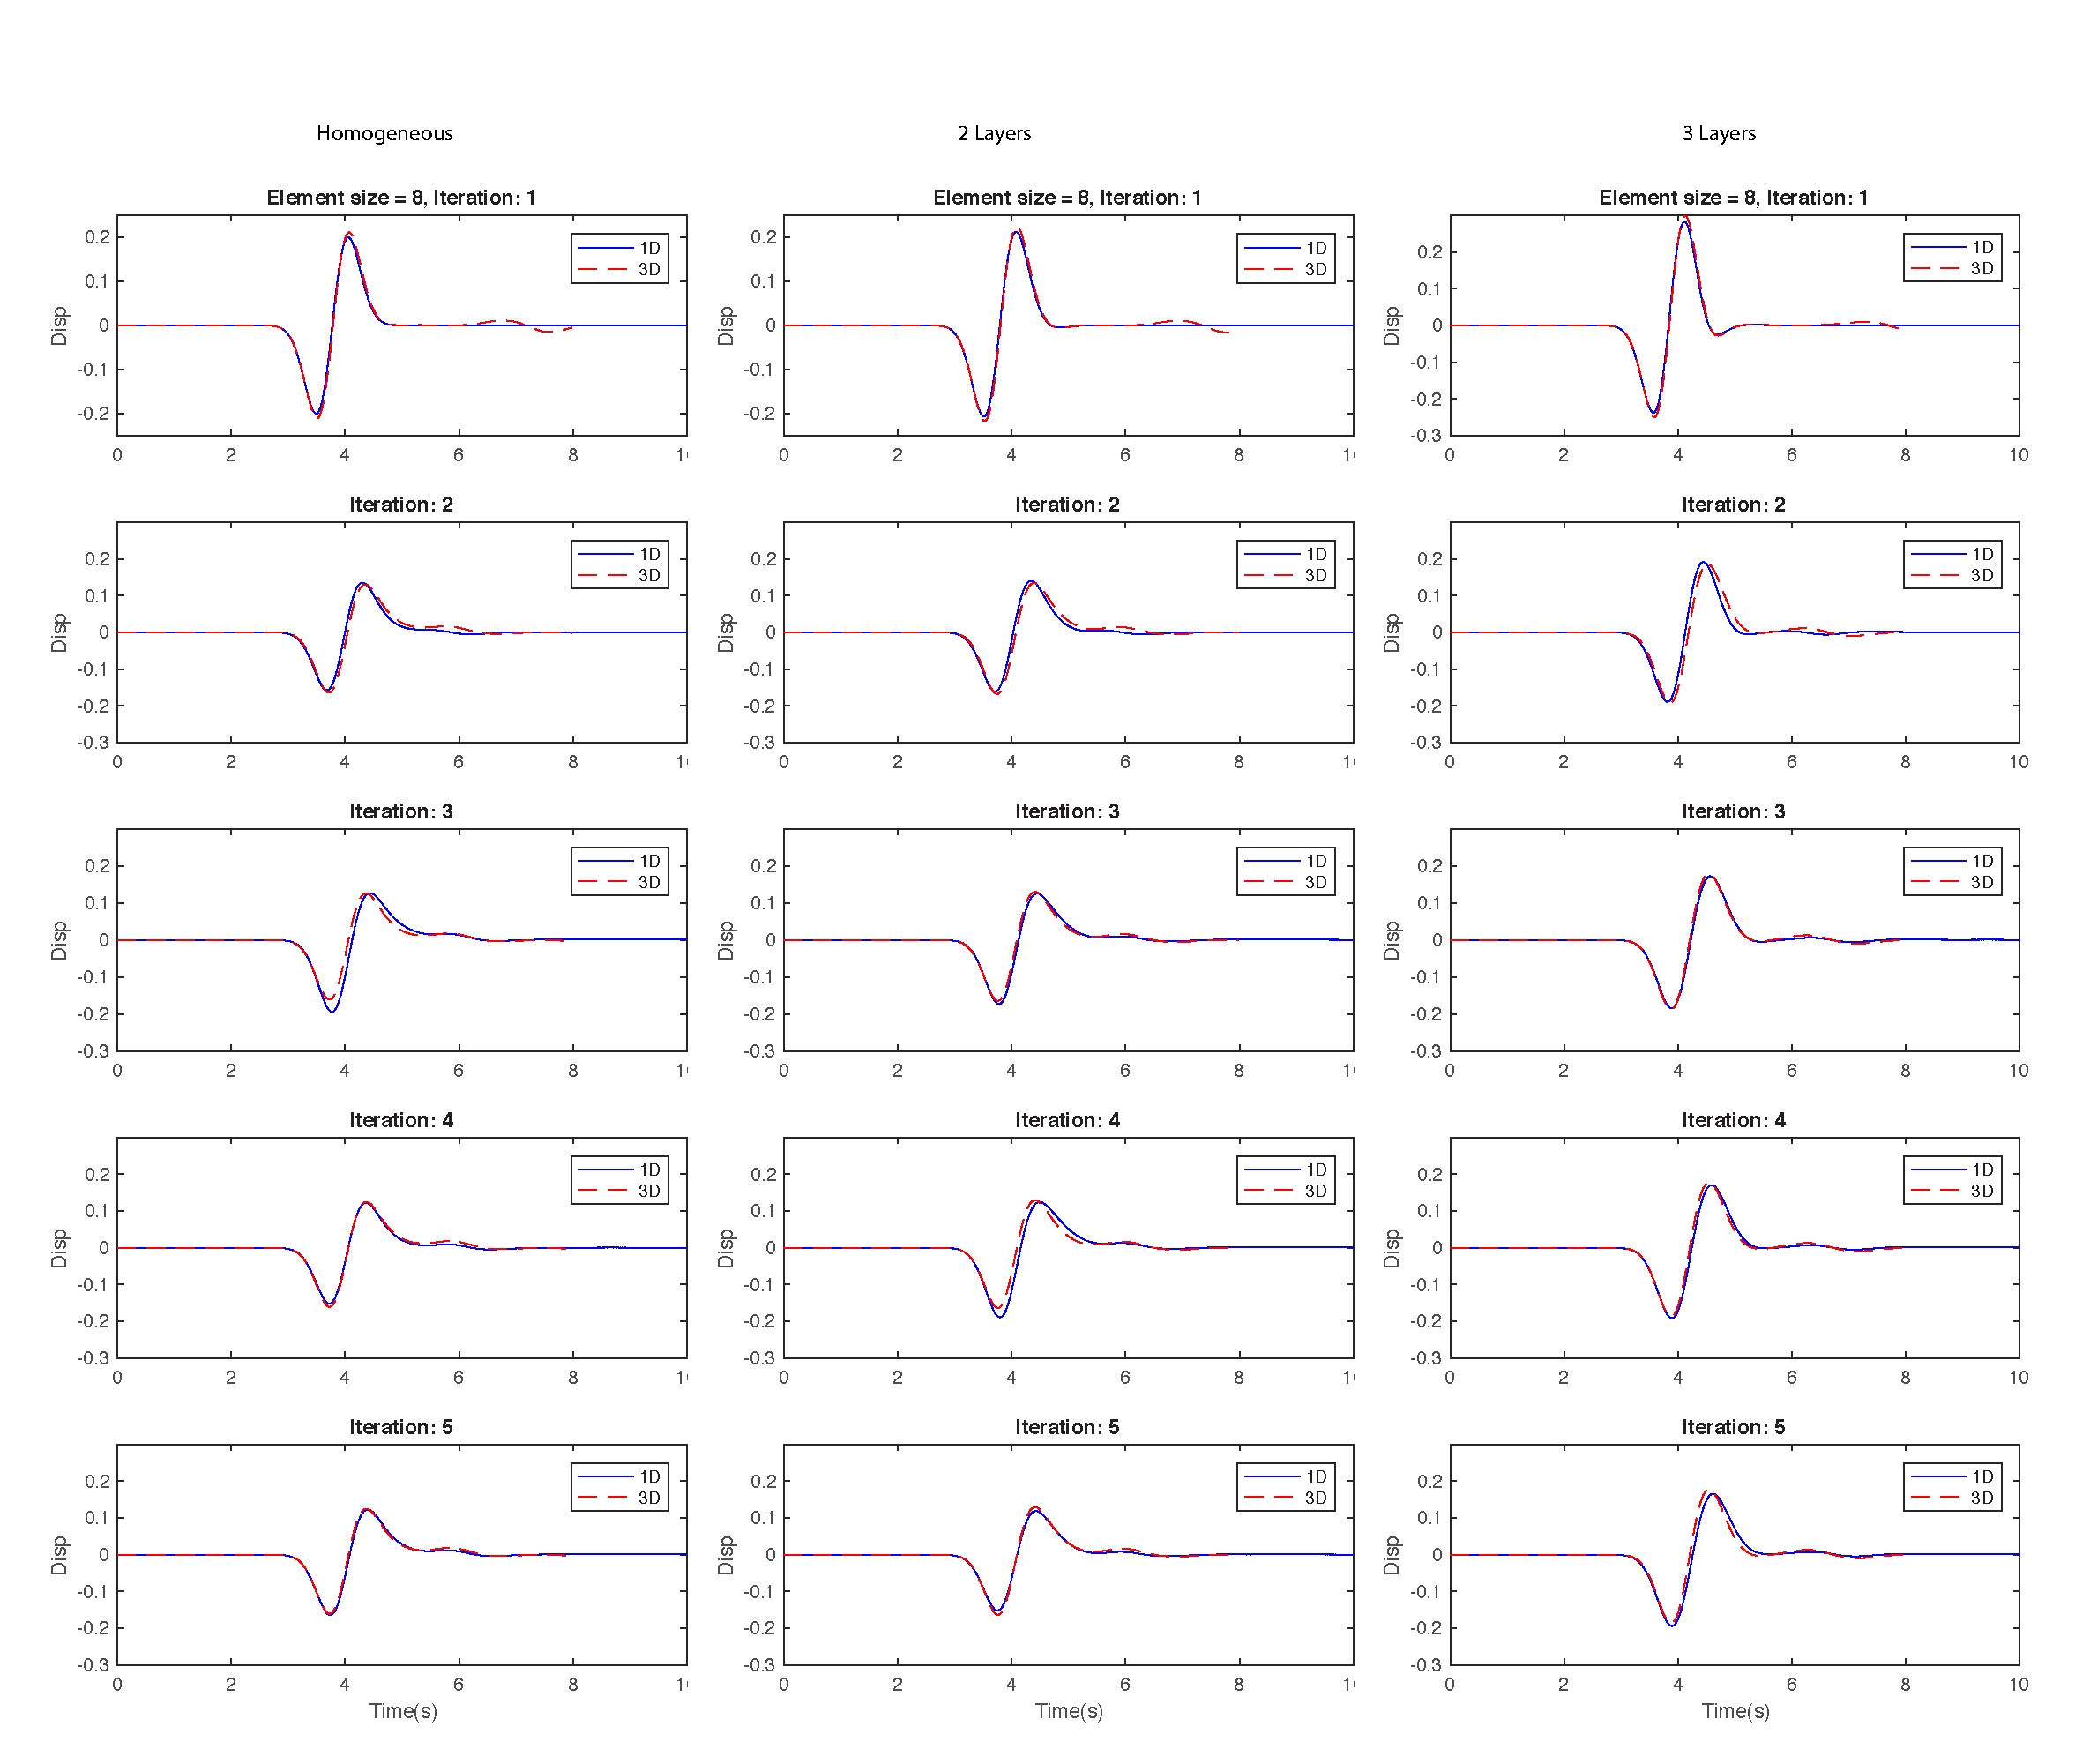
\includegraphics[width=\textwidth]{figures/pdf/comparison_1D_3D_3models_results.pdf}
    \caption{Comparison of displacement at the surface station for 1D and 3D simulation. Simulation is done for one sided horizontal wave propagation in 3D domain and 1D domain. The 0.1 displacement is applied at the bottom of the domain at the DRM elements.}
    \label{fig:comparison_1D_3D_3models_results}
\end{figure}

The strain values are computed through the following equation and only updated for $\epsilon_{xz} $ values.

%\begin{equation}
%\epsilon = \begin{bmatrix}
%\epsilon_{xx} &\epsilon_{xy}  &\epsilon_{xz} \\ 
%\epsilon_{yx} &\epsilon_{yy}  &\epsilon_{yz} \\ 
%\epsilon_{zx} &\epsilon_{zy}  &\epsilon_{zz} 
%\end{bmatrix} =
%\begin{bmatrix}
%\epsilon_{xx} &\frac{1}{2}\gamma_{xy}  &\frac{1}{2}\gamma_{xz} \\ 
%\frac{1}{2}\gamma_{yx} &\epsilon_{yy}  &\frac{1}{2}\gamma_{yz} \\ 
%\frac{1}{2}\gamma_{zx} &\frac{1}{2}\gamma_{zy}  &\epsilon_{zz} 
%\end{bmatrix},
%\end{equation}

where

\begin{equation}
\gamma_{xy}=\alpha + \beta = \frac{\partial u_y}{\partial x} + \frac{\partial u_x}{\partial y}
\end{equation}

The force is the integration of a Ricker pulse which is applied through DRM method. Fig.~\ref{fig:DRM_schematic} shows the schematic of the force application. 

 \begin{figure}
    \centering
    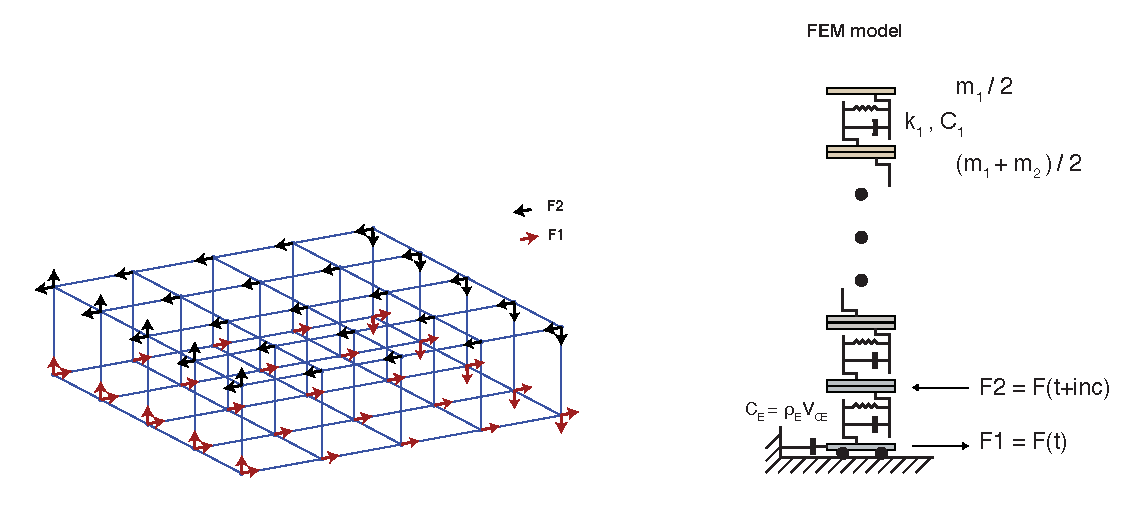
\includegraphics[width=\textwidth]{figures/pdf/DRM_schematic.pdf}
    \caption{Schematic of application of force using DRM method for 3D and 1D domain.}
    \label{fig:DRM_schematic}
\end{figure}
